\documentclass[11pt]{article}
\usepackage{color, array, graphics}
\usepackage{amsmath}
\usepackage{amssymb}
\usepackage{enumerate}
\usepackage{mathtools}
\usepackage{fullpage}
\usepackage{graphicx}
\usepackage{float}
\usepackage[utf8]{inputenc}

%Symbol shortcuts
\def\OR{\vee}
\def\AND{\wedge}
\def\imp{\rightarrow}


\begin{document}

\begin{center} Alexander Garcia \hfill June 5, 2017 \\ Assignment-2 \end{center}

\medskip

\begin{enumerate}

\item

	\begin{enumerate}[(a)]

		\item Consider the functions $f(x) = x^3 - 2,\ g(x) = e^x - 5sin(x^3) - 3cos(x)$. \\

		The initial step in the bisection process is to choose a range of $x$ in which $f(x) = 0$. As the range is given to be $(0,2)$,
		the bisection algorithm proceeds by guessing the midpoint of the range (let's call this $x_0 = \frac{b_0-a_0}{2}$) to be a zero
		of the function. If $|f(x_0)| \leq 0 + tol$, then the zero is said to have been found. If $|f(x_0)| > 0 + tol$, then either
		$a_0$ or $b_0$ is replaced by $x_0$, depending on where $f(x)$ changes sign. The process is then repeated until
		$f(x_n) < 0 + tol$. \\

		At each stage in the algorithm, the maximum possible error of $f(x_n)$ is $e_n = \frac{b_n-a_n}{2}$, and the general error is
		$e_n \leq \frac{b_n-a_n}{2}$. Because $b_n-a_n = \frac{b_{n-1}-a_{n-1}}{2}$, we can express the current error as
		$$e_n \leq \frac{1}{2} e_{n-1}$$

		In this case we are taking 34 iterations until $e_n$ is reasonably low, so $e_{34} = \frac{1}{2} e_{33}$. It is clear that this
		expression will cascade down to $e_0$, the error of the initial guess. The final error $e_{34}$ can therefore be generalized
		to
		$$e_0*\prod_{i = 1}^{34}\frac{1}{2} = 1*\prod_{i=1}^{34}\frac{1}{2} = \frac{1}{2^{34}} $$

		This result shows that the errors of the bisection method do not rely at all upon the function whose zeroes are being
		calculated, but rather solely upon the number of iterations carried out by the process. The number of iterations to calculate
		$g(x) = 0$ to sufficent accuracy is exactly the same number of iterations needed to calculate $f(x) = 0$. \\

		\item The convergence rate of a root finding algorithm is the limit of the ratio of the error in iteration $n$ to the error in
		iteration $n-1$ as $n \rightarrow \infty$.
		$$conv = \lim_{n\to\infty} \frac{e_n}{e_{n-1}}$$

		\begin{enumerate}[i.]

			\item This algorithm is linearlly convergent, or has a constant convergance rate, as the ratio between every adjacent
			error is $\frac{1}{2}$.

			\item This algorithm is quadratically convergent. It is clear that the ratio of $e_n$ to $e_{n-1}$ is cut in half
			after every iteration, making the rate of convergance not a constant factor, but a result of which iteration is
			currently taking place.
			$$(\frac{e_n}{e_{n-1}} = \frac{1}{2^n})|_{n=1}^{\infty}$$ \\

		\end{enumerate}

		\item For a ``good'' starting guess when undergoing Newton approximation, the rate of convergence is quadratic. \\

			After choosing a good starting guess, the next approximations for $f(x)=0$ are determined by $x_{n+1} = x_n-\frac{f(x_n)}{f^{'}(x_n)}$, where
			$x_n$ approaches the true zero, $x=\alpha$. At each stage, the error is $e_n = |x_n-\alpha|$, and the rate of convergance would be
			$\frac{e_n}{e_{n+1}}$. \\

			We let the function $f(x)$ be approximated by the first order Taylor polynomial about $x_n$.
			$$f(x) = f(x_n) + (x-x_n)f^{'}(x_n) + \frac{1}{2} (x-x_n)^2f^{''}(c_n)$$
			where $c_n$ is a constant close to $x_n$ used to estimate the remainder. If we evaluate the approximation at $x=\alpha$, we would ideally get zero,
			as this is the true root of the function.
			$$0 = f(x_n) + (\alpha - x_n)f^{'}(x_n) + \frac{1}{2} (\alpha-x_n)^2f^{''}(c_n)$$
			If we then divide by $f^{'}(x_n)$, we see that the expression for $x_{n+1}$ appears.
			$$0 = \frac{f(x_n)}{f^{'}(x_n)}+(\alpha-x_n) + \frac{(\alpha-x_n)^2}{2} \frac{f^{''}(c_n)}{f^{'}(x_n)} $$
			$$x_n - \frac{f(x_n)}{f^{'}(x_n)} - \alpha = \frac{(\alpha-x_n)^2}{2} \frac{f^{''}(c_n)}{f^{'}(x_n)} $$
			$$x_{n+1}-\alpha = \frac{1}{2} (\alpha - x_n)^2 \frac{f^{''}(c_n)}{f^{'}(x_n)} $$
			We know that by definition, $x_n-\alpha = e_n$, and that $\lim_{n\to\infty}x_n = \alpha$,  so this can be rewritten as
			$$\frac{e_{n+1}}{{e_n}^2} = \frac{1}{2}\frac{f^{''}(\alpha)}{f^{'}(\alpha)} $$
			Because the right hand side is constant, and the ratio of errors is of the form $\frac{R}{R^2} = c$, we can say that the sequence is
			quadratically convergant. \\

			If a poor starting guess is chosen, Newton's method will not converge at all towards a root of the function. A ``bad'' starting guess would be in
			the region [a,b] about the root such that

			\begin{itemize}
				\item $f,f^{'}, f^{''}$ does not exist in [a,b]
				\item $f^{'} = 0$ in [a,b]
				\item $f^{''}$ changes sign in [a,b] \\
			\end{itemize}

			\begin{center}
				Therefore, \textbf{ii and iii} are correct. \\
			\end{center}

			\newpage

		\item True. If an initial guess for Newton's root finding method is to be considered ``good'', it must follow some criteron.
		\begin{itemize}
			\item $f, f^{'}, f^{''}$ must exist exist

			\item Choose $a,b$ such that $f(a)*f(b)<0$

			\item $f^{'} \neq 0$ in $[a,b]$

			\item $f^{''}$ does not change sign in $[a,b]$

			\item $|\frac{f(a)}{f^{'}(a)}|$ and $|\frac{f(b)}{f^{'}(b)}| < |b-a|$
		\end{itemize}

		If all of these hold true, the there will be a unique root in $[a,b]$, and any starting guess in $[a,b]$ will
		converge to the root. Therefore, if $x_0$ leads to convergance, then any guess between $x^*$ and $x_0$ will also
		lead to convergance. \\

		\item One of the main advantages of Newton's method over the bisection method is the speed at which it can approximate roots.
		The quadratic convergance rate of Newton's method means that given a good starting guess, it can approximate a root in a
		fraction of the time of the bisection method.

		However, unlike the bisection method, it requires a good starting guess. If
		the initial zero chosen does not follow some precise specifications (see part(d)), then the method will not converge. Despite
		its much longer runtime, the bisection method will always work, given that $\alpha$ lies in the initial range.

		Also, Newton's method can be somewhat more difficult to compute, as the $f^{'}$ is needed to compute the root of $f$. The
		bisection method relies solely on $f$. \\

		\item One of the main advantages of the Secant method over Newton's method is the fact that the secant method does not require
		$f^{'}(x)$ to approximate the root. However, it requires two starting guesses, and does not converge at the rate of
		Newton's method (Newton's: quadratic convergance, secant: ``superlinear'' convergance).


		\item $f(x) = 2-x^2$

		$f^{'}(x) = -2x$

		We choose $x_0=2$ for a starting guess. \\

		The rule for Newton's method is $x_{n+1} = x_n-\frac{f(x_n)}{f^{'}(x_n)}$ \\

		$x_1 = x_0 - \frac{f(x_0)}{f^{'}(x_0)} = \frac{3}{2}$ \\

		$x_2 = x_1 - \frac{f(x_1)}{f^{'}(x_1)} = \frac{17}{12}$ \\

		$x_3 = x_2 - \frac{f(x_2)}{f^{'}(x_2)} = \frac{577}{408}$ \\

		$x_4 = x_3 - \frac{f(x_3)}{f^{'}(x_3)} = \frac{665857}{470832}$ \\

		$x_5 = x_4 - \frac{f(x_4)}{f^{'}(x_4)} = \frac{886731088897}{627013566048}$ \\

		At this point, if we define the tolerance as $10^{-12}$, we must see if we are close enough to the root. Because technically
		we do not know the true answer $\sqrt{2}$, we see if the last two roots are sufficiently close together.

		$x_5 - x_4 = \frac{665857}{470832} - \frac{886731088897}{627013566048} = \frac{1}{627013566048} \approx 1.6*10^{-12}$

		The result is within the defined tolerance, and the algorithm is complete, with the calculated root being
		$$x_5 = \frac{886731088897}{627013566048} \approx 1.41421356237468$$

		Compared to the actual value of the root, $\sqrt{2}$, the relative error is
		$\frac{x_5 - \sqrt{2}}{\sqrt{2}} \approx 1.13*10^{-12}$ \\

		\item The bisection method will not converge to a real number answer. The rule of the bisection method is that you begin by
		defining a domain in which the root lies, which is done by checking where $f(x)$ changes sign. In the case of
		$f(x) = \frac{1}{x} $, the function only changes sign if the lower bound ($x=a$) is less than zero, and the upper bound
		($x=b$) is greater than zero.

		As this is the only possible point the zero could be, the bisection algorithm will keep approaching the midpoint of
		[a,b], which will approach zero. But as we know,
		$\frac{1}{0+\delta}$ becomes increasingly large as $\delta \to 0$.

		Therefore, the bisection method will not converge to a real number answer, which is good, since there are no real number
		answers to $\frac{1}{x} = 0$. \\

		\begin{figure}[H]
			\centering
			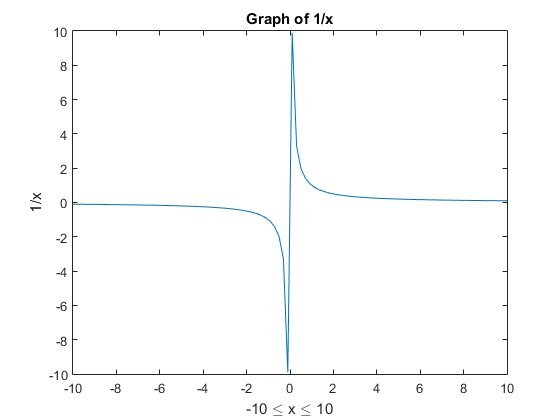
\includegraphics[width=0.6\textwidth]{q1i.png}
			\caption{Graph of $\frac{1}{x}$ produced by MATLAB}
		\end{figure}

		\item
		\begin{enumerate}[i.]
		\item $f(x) = x^2sinx^2$

		$f(x) = (x-r)^m*F(x)$

		The exponent on the $(x-r)$ term of the function is, by definition, the multiplicity of the root $r$. In this case
		the multiplicity of root $r = 0$ is 2.

		\item Assume we are using Newton's method for root finding. The next approximated zero is defined as $x_{n+1} =
			x_n - \frac{f(x_n)}{f^{'}(x_n)}$.

			If $f^{'}(x) >> 1$ as the approximation approaches the root, then we should
			use the $f(x_n)$ as the stopping criteria, since if $f^{'}(x_n)$ grows too large, we lose the significance of the
			result $(\frac{f(x_n)}{f^{'}(x_n)} \approx 0)$.

			If $f^{'}(x_n) << 1$, we should approximate the zero as $x_{n+1}-
			x_n$, since a large $f^{'}(x_n) \to \frac{f(x_n)}{f^{'}(x_n)} \approx \infty$, which again removes significance
			from the result. \\

			In this case, $f^{'}(x) = 2xsinx^2 + x^2cosx^2$. As $x\to0$, the function will grow increasingly small. Therefore,
			we should accept the result when $|x_{n+1} - x_n| < tol$. \\
		\end{enumerate}

	\end{enumerate}

\item Holmes 2.4 (B)

	\begin{enumerate}[(a)]

		\item See Figure 2
			\begin{figure}[H]
			\centering
			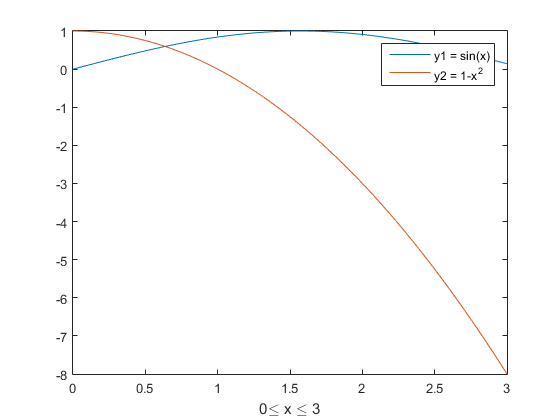
\includegraphics[width=0.6\textwidth]{q2_graph.png}
			\caption{Graph of $sinx$ and $1-x^2$}
		\end{figure}

		\item We can treat the equation $sinx = 1-x^2$ as $sinx + x^2 - 1 = 0$, where we are solving for the roots of the function.
		It is clear that the intersection of the two points occurrs somewhere between $x=0.5$ and $x=1$, so we choose $a = 0.5$ and
		$b=1$. We can see that the root lies within this range, since $f(0.5) \approx -0.27057\dots$, and $f(1) \approx 0.84147\dots$,
		meaning that $f(a) * f(b) < 0$. We have shown that the function changes sign in this interval, and according to the
		Intermediate Value Theorem, if a function is continuous over an interval, then the function must take every value between
		$(f(a), f(b)$. In this case, it means that if a function is negative on one end of the interval and positive on the other,
		the zero must lie somewhere in the interval.\\

		The initial guess, $c_0$ would simply be the midpoint of $a$ and $b$.
		$$c_0 = \frac{b+a}{2} = \frac{1.5}{2} = 0.75$$

		We must then test to see whether $a$ is replaced by $c_0$, or if $b$ is replaced by $c_0$.
		$$f(c_0) \approx 0.24414\dots$$

		Because the root must lie in the domain where $f(x)$ changes signs, we must replace $a$ with $c_0$, as $f(a) > 0$.

		We now repeat the process to find $c_1$
		$$c_1 = \frac{b+c_0}{2} = \frac{1.25}{2} = 0.625$$

		\item The general form for each iteration of Newton's method is
		$$x_{n+1} = x_n - \frac{f(x_n)}{f^{'}(x_n)} $$
		In this case, $f(x) = sinx + x^2 - 1$, and $f^{'}(x) = cosx + 2x$. The only element left is $x_0$. This must be chosen
		carefully, as a poor initial guess will not lead to convergance. A good guess will follow the rules outlined in Question 1
		part (d). As a quick check,

		\begin{itemize}
			\item $f(x) = sinx + x^2 - 1,\ f^{'}(x) = cosx+2x,\ f^{''}(x) = 2-sinx$

			\item If $a = 0$ and $b=1$, we can see that $f(a) = -1,\ f(b) = sin(1)$, so $f(a)*f(b) < 0$. This means there is a
			root in the range $[a,b]$.

			\item As shown in Figure 3, the first derivative of $f(x)$ is nonzero for all $0 \leq x \leq 1$.

			\item As shown in Figure 3, the second derivative of $f(x)$ is positive for all $0 \leq x \leq 1$.

			\item $|\frac{f(a)}{f^{'}(a)}| = \frac{1}{1} \leq 1-0$

			$|\frac{f(b)}{f^{'}(b)}| = \frac{sin(1)}{cos(1) + 2} \approx 0.33125 \leq 1-0$

		\end{itemize}

		\begin{figure}[H]
			\centering
			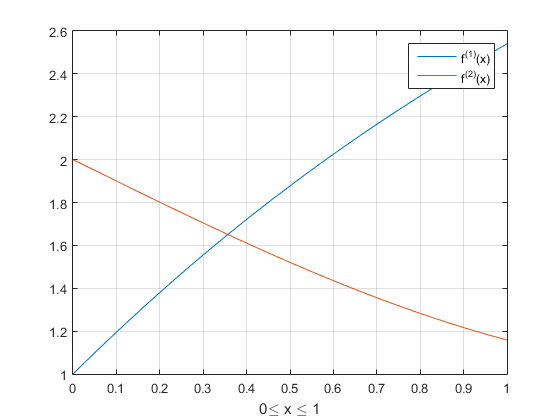
\includegraphics[width=0.6\textwidth]{q2_derivgraph.png}
			\caption{Graph of $f^{'}(x)$ and $f^{''}(x)$}
		\end{figure}

		We can now proceed with a starting guess anywhere in the range $0 \leq x_0 \leq 1$. As it is the easiest, choose $x_0 = 0$.

		$$x_1 = 0 - \frac{f(0)}{f^{'}(0)} = -\frac{-1}{1} = 1$$

		\item The general form for the secant method is
			$$x_{n+2} = x_{n} - \frac{f(x_n)(x_{n+1}-x_n)}{f(x_{n+1})-f(x_n)} = x_n - \frac{f(x_n)}{m_n} $$

			A good choice for starting points $x_0, x_1$ would be points close to the true root of $f(x)$ which will lead the
			algorithm to convergance.

			More formally, let us let $f(\overline{x})=0$. If $f(x)$ is twice differentiable in
			$a < \overline{x} < b$ and $f^{'}(x) \neq 0$ in $(a,b)$, then any $x_0, x_1$ chosen close to $\overline{x}$ will
			converge to $\overline{x}$ through the secant method. \\

			As the root of this function is $0 < \overline{x} < 1$, we can choose $x_0 = 1, x_1 = 0$.
			$$x_2 = 1 - \frac{f(1)(0-1)}{f(0)-f(1)} = 1- \frac{-sin(1)}{-1-sin(1)} \approx 0.54304$$

		\item In order to compute the exact solution to the equation, I used a MATLAB script defining Newton's Method. I chose this
			method as it converges the fastest out of the three algorithms, and only requires a single starting guess. For error,
			I used $10^{-15}$ as the stopping criteria. All credit for the MATLAB script goes to professor Kapila.

			$$\overline{x} = 0.6367$$

			\begin{figure}[H]
				\centering
				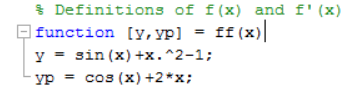
\includegraphics[width=0.4\textwidth]{q2_fundef.PNG}
				\caption{Definition of $f(x)$ and $f'(x)$}
			\end{figure}

			\begin{figure}[H]
				\centering
				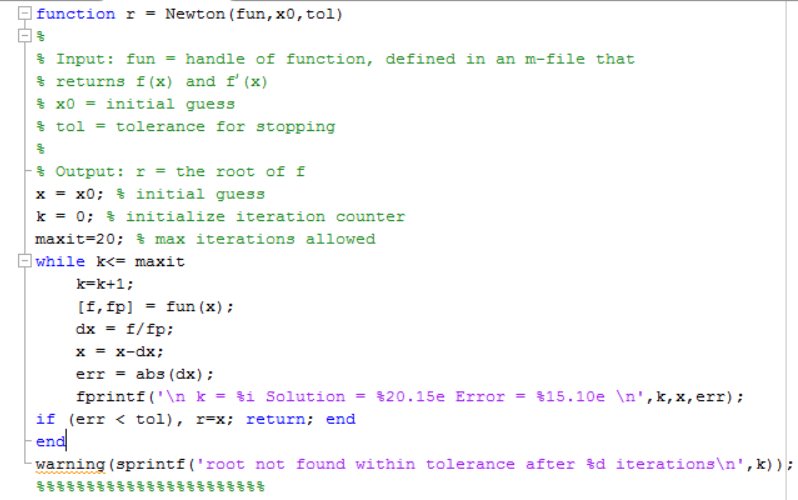
\includegraphics[width=\textwidth]{q2_newtonscript.PNG}
				\caption{Script used to calculate $\overline{x}$}
			\end{figure}

			\begin{figure}[H]
				\centering
				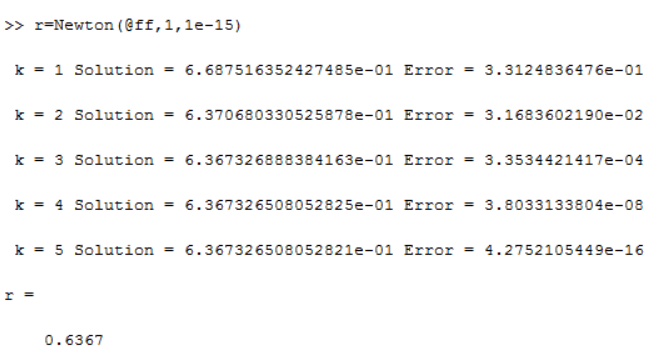
\includegraphics[width=0.8\textwidth]{q2_out.PNG}
				\caption{Printed output of script in Figure 5}
			\end{figure}
	\end{enumerate}

\item
\end{enumerate}

\end{document}


